\documentclass[tikz,border=6pt]{standalone}
\usepackage{amsmath,amssymb}
\usetikzlibrary{arrows.meta,positioning,calc}

\begin{document}
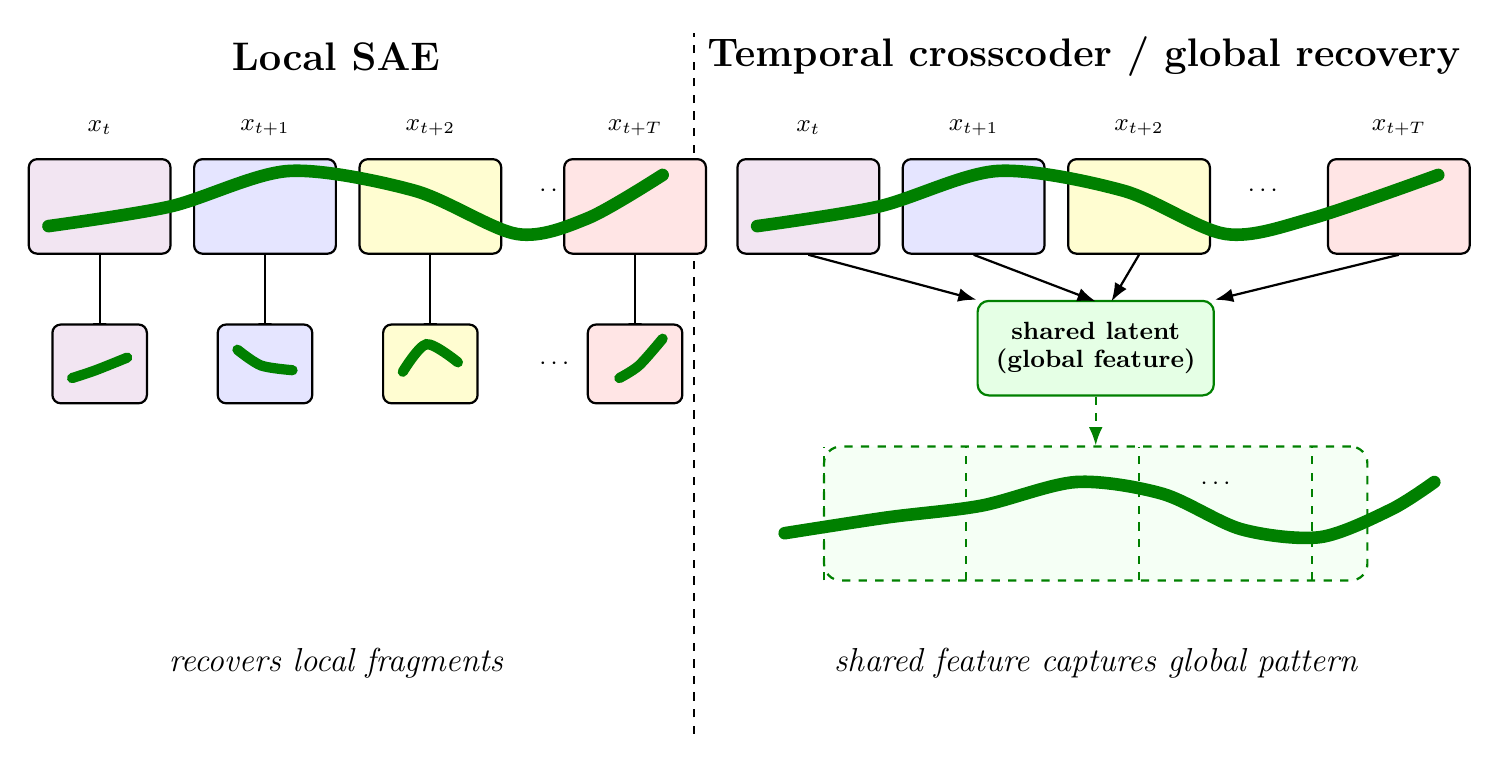
\begin{tikzpicture}[
    >=Latex,
    font=\small,
    line width=0.8pt,
    every node/.style={align=center},
    actboxA/.style={draw, rounded corners=3pt, minimum width=1.8cm, minimum height=1.2cm, fill=violet!10},
    actboxB/.style={draw, rounded corners=3pt, minimum width=1.8cm, minimum height=1.2cm, fill=blue!10},
    actboxC/.style={draw, rounded corners=3pt, minimum width=1.8cm, minimum height=1.2cm, fill=yellow!18},
    actboxD/.style={draw, rounded corners=3pt, minimum width=1.8cm, minimum height=1.2cm, fill=red!10},
    fragboxA/.style={draw, rounded corners=3pt, minimum width=1.2cm, minimum height=1.0cm, fill=violet!10},
    fragboxB/.style={draw, rounded corners=3pt, minimum width=1.2cm, minimum height=1.0cm, fill=blue!10},
    fragboxC/.style={draw, rounded corners=3pt, minimum width=1.2cm, minimum height=1.0cm, fill=yellow!18},
    fragboxD/.style={draw, rounded corners=3pt, minimum width=1.2cm, minimum height=1.0cm, fill=red!10},
    latentbox/.style={draw, rounded corners=4pt, minimum width=3.0cm, minimum height=1.2cm, fill=green!10, draw=green!50!black},
    globalbox/.style={draw, rounded corners=6pt, dashed, minimum width=6.9cm, minimum height=1.7cm, fill=green!4, draw=green!50!black},
    title/.style={font=\bfseries\Large},
    subtitle/.style={font=\itshape\large}
]

% -------------------------------------------------
% TITLES
% -------------------------------------------------
\node[title] at (3.8, 4.8) {Local SAE};
\node[title] at (13.3, 4.8) {Temporal crosscoder / global recovery};

% -------------------------------------------------
% VERTICAL DIVIDER
% -------------------------------------------------
\draw[dashed] (8.35, -3.8) -- (8.35, 5.1);

% =================================================
% LEFT PANEL
% =================================================

% top labels
\node at (0.8, 3.9) {$x_t$};
\node at (2.9, 3.9) {$x_{t+1}$};
\node at (5.0, 3.9) {$x_{t+2}$};
\node at (6.6, 3.1) {$\cdots$};
\node at (7.6, 3.9) {$x_{t+T}$};

% top boxes
\node[actboxA] (L1) at (0.8, 2.9) {};
\node[actboxB] (L2) at (2.9, 2.9) {};
\node[actboxC] (L3) at (5.0, 2.9) {};
\node[actboxD] (L4) at (7.6, 2.9) {};

% green global pattern through top
\draw[green!50!black, line width=1.6mm, line cap=round]
    plot[smooth] coordinates {
        (0.15,2.65) (1.7,2.9) (3.2,3.35) (4.8,3.1)
        (6.1,2.55) (7.0,2.75) (7.95,3.3)
    };

% arrows to local fragments
\draw[->] (L1.south) -- ++(0,-1.1);
\draw[->] (L2.south) -- ++(0,-1.1);
\draw[->] (L3.south) -- ++(0,-1.1);
\draw[->] (L4.south) -- ++(0,-1.1);

% bottom local fragment boxes
\node[fragboxA] (LF1) at (0.8, 0.9) {};
\node[fragboxB] (LF2) at (2.9, 0.9) {};
\node[fragboxC] (LF3) at (5.0, 0.9) {};
\node at (6.6, 0.9) {$\cdots$};
\node[fragboxD] (LF4) at (7.6, 0.9) {};

% fragment curves
\draw[green!50!black, line width=1.3mm, line cap=round]
    plot[smooth] coordinates {(0.45,0.72) (0.75,0.82) (1.15,0.98)};
\draw[green!50!black, line width=1.3mm, line cap=round]
    plot[smooth] coordinates {(2.55,1.08) (2.85,0.88) (3.25,0.82)};
\draw[green!50!black, line width=1.3mm, line cap=round]
    plot[smooth] coordinates {(4.65,0.8) (4.95,1.15) (5.35,0.92)};
\draw[green!50!black, line width=1.3mm, line cap=round]
    plot[smooth] coordinates {(7.4,0.72) (7.65,0.88) (7.95,1.22)};

% left subtitle
\node[subtitle] at (3.8, -2.9) {recovers local fragments};

% =================================================
% RIGHT PANEL
% =================================================

% top labels
\node at (9.8, 3.9) {$x_t$};
\node at (11.9, 3.9) {$x_{t+1}$};
\node at (14.0, 3.9) {$x_{t+2}$};
\node at (15.6, 3.1) {$\cdots$};
\node at (17.3, 3.9) {$x_{t+T}$};

% top boxes
\node[actboxA] (R1) at (9.8, 2.9) {};
\node[actboxB] (R2) at (11.9, 2.9) {};
\node[actboxC] (R3) at (14.0, 2.9) {};
\node[actboxD] (R4) at (17.3, 2.9) {};

% green pattern through top
\draw[green!50!black, line width=1.6mm, line cap=round]
    plot[smooth] coordinates {
        (9.15,2.65) (10.7,2.9) (12.2,3.35) (13.8,3.1)
        (15.1,2.55) (16.2,2.75) (17.8,3.3)
    };

% shared latent box
\node[latentbox] (latent) at (13.45, 1.1) {\textbf{shared latent}\\[-1pt]\textbf{(global feature)}};

% arrows from top boxes to latent
\draw[->] (R1.south) -- (latent.north west);
\draw[->] (R2.south) -- ($(latent.north)+(0,-0.02)$);
\draw[->] (R3.south) -- ($(latent.north)+(0.2,-0.02)$);
\draw[->] (R4.south) -- (latent.north east);

% bottom global box
\node[globalbox] (global) at (13.45, -1.0) {};

% dashed arrow from latent to global
\draw[->, dashed, draw=green!50!black] (latent.south) -- (global.north);

% optional dashed separators in global box
\draw[dashed, draw=green!50!black] (10.0,-1.85) -- (10.0,-0.15);
\draw[dashed, draw=green!50!black] (11.8,-1.85) -- (11.8,-0.15);
\draw[dashed, draw=green!50!black] (14.0,-1.85) -- (14.0,-0.15);
\draw[dashed, draw=green!50!black] (16.2,-1.85) -- (16.2,-0.15);

% global recovered curve
\draw[green!50!black, line width=1.6mm, line cap=round]
    plot[smooth] coordinates {
        (9.5,-1.25) (10.8,-1.05) (12.0,-0.9) (13.2,-0.6)
        (14.3,-0.75) (15.3,-1.2) (16.3,-1.3) (17.2,-0.95) (17.75,-0.6)
    };

\node at (15.0,-0.63) {$\cdots$};

% right subtitle
\node[subtitle] at (13.45, -2.9) {shared feature captures global pattern};

\end{tikzpicture}
\end{document}